\hypertarget{a00002}{
\section{eqOsg::Channel Class Reference}
\label{a00002}\index{eqOsg::Channel@{eqOsg::Channel}}
}
The \hyperlink{a00002}{Channel} renders the frames in \hyperlink{a00002_70cfd22742da9b9aa3e3478f356ba220}{frameDraw()}.  


{\tt \#include $<$Channel.h$>$}

Collaboration diagram for eqOsg::Channel:\nopagebreak
\begin{figure}[H]
\begin{center}
\leavevmode
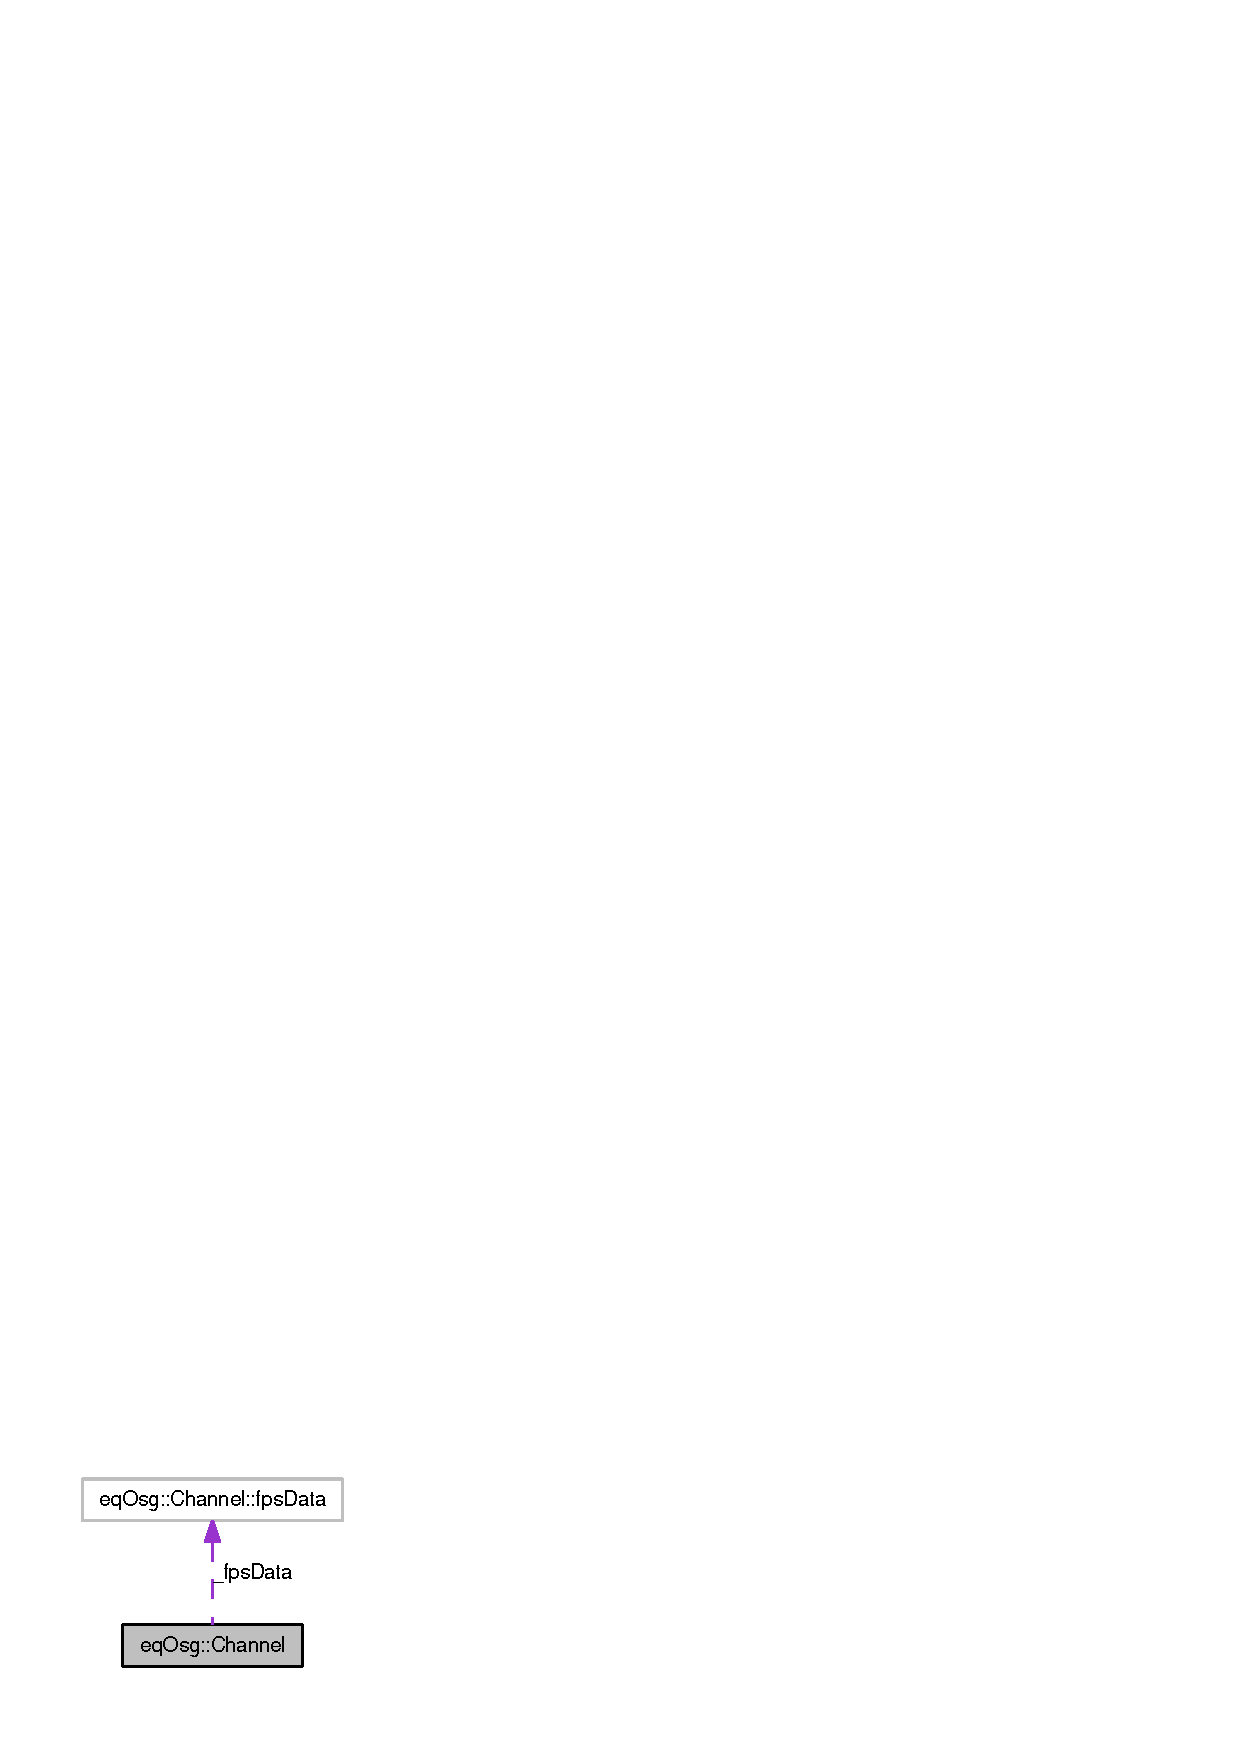
\includegraphics[width=168pt]{a00087}
\end{center}
\end{figure}
\subsection*{Classes}
\begin{CompactItemize}
\item 
struct \textbf{fpsData}
\begin{CompactList}\small\item\em framecounter stuff \item\end{CompactList}\end{CompactItemize}
\subsection*{Public Member Functions}
\begin{CompactItemize}
\item 
\hyperlink{a00002_332b524bf3dd36fb43ff699fb8b64052}{Channel} (eq::Window $\ast$parent)
\begin{CompactList}\small\item\em Creates a channel and sets its parent window. \item\end{CompactList}\end{CompactItemize}
\subsection*{Protected Member Functions}
\begin{CompactItemize}
\item 
virtual void \hyperlink{a00002_70cfd22742da9b9aa3e3478f356ba220}{frameDraw} (const uint32\_\-t frameID)
\begin{CompactList}\small\item\em Renders the scene graph. \item\end{CompactList}\item 
virtual bool \hyperlink{a00002_15ff8d6c9962d86d886dba9485082dde}{configInit} (const uint32\_\-t initID)
\begin{CompactList}\small\item\em \hyperlink{a00003}{Config} initialisation. \item\end{CompactList}\item 
osg::Matrix \hyperlink{a00002_d3a369c393e8065327ef37cef65e25c7}{setPlainViewMatrix} (const \hyperlink{a00014}{Pipe} $\ast$frameData) const 
\begin{CompactList}\small\item\em This function gets the camera position and viewing direction information out of the frame data and sets the view matrix of the camera of the viewer of the pipe based on this information. \item\end{CompactList}\item 
\hypertarget{a00002_2950f8b33948b9f8fea20910b95fc695}{
virtual void \hyperlink{a00002_2950f8b33948b9f8fea20910b95fc695}{drawFPS} ()}
\label{a00002_2950f8b33948b9f8fea20910b95fc695}

\begin{CompactList}\small\item\em Prints the self calculated FPS value. \item\end{CompactList}\item 
\hypertarget{a00002_e0efffd06ae7a755b7f0c80641d5e6d7}{
virtual void \hyperlink{a00002_e0efffd06ae7a755b7f0c80641d5e6d7}{drawInfoText} (std::string txt)}
\label{a00002_e0efffd06ae7a755b7f0c80641d5e6d7}

\begin{CompactList}\small\item\em Prints the channel's info Text. \item\end{CompactList}\end{CompactItemize}


\subsection{Detailed Description}
The \hyperlink{a00002}{Channel} renders the frames in \hyperlink{a00002_70cfd22742da9b9aa3e3478f356ba220}{frameDraw()}. 

This is done by querying the pipe for the viewer and then asking the viewer to render the scene. 

\subsection{Constructor \& Destructor Documentation}
\hypertarget{a00002_332b524bf3dd36fb43ff699fb8b64052}{
\index{eqOsg::Channel@{eqOsg::Channel}!Channel@{Channel}}
\index{Channel@{Channel}!eqOsg::Channel@{eqOsg::Channel}}
\subsubsection[{Channel}]{\setlength{\rightskip}{0pt plus 5cm}Channel::Channel (eq::Window $\ast$ {\em parent})}}
\label{a00002_332b524bf3dd36fb43ff699fb8b64052}


Creates a channel and sets its parent window. 

\begin{Desc}
\item[Parameters:]
\begin{description}
\item[{\em parent}]The equalizer parent window. \end{description}
\end{Desc}


\subsection{Member Function Documentation}
\hypertarget{a00002_15ff8d6c9962d86d886dba9485082dde}{
\index{eqOsg::Channel@{eqOsg::Channel}!configInit@{configInit}}
\index{configInit@{configInit}!eqOsg::Channel@{eqOsg::Channel}}
\subsubsection[{configInit}]{\setlength{\rightskip}{0pt plus 5cm}bool Channel::configInit (const uint32\_\-t {\em initID})\hspace{0.3cm}{\tt  \mbox{[}protected, virtual\mbox{]}}}}
\label{a00002_15ff8d6c9962d86d886dba9485082dde}


\hyperlink{a00003}{Config} initialisation. 

\begin{Desc}
\item[Parameters:]
\begin{description}
\item[{\em initID}]The initID of the config. \end{description}
\end{Desc}
\begin{Desc}
\item[Returns:]True if succeed. \end{Desc}
\hypertarget{a00002_70cfd22742da9b9aa3e3478f356ba220}{
\index{eqOsg::Channel@{eqOsg::Channel}!frameDraw@{frameDraw}}
\index{frameDraw@{frameDraw}!eqOsg::Channel@{eqOsg::Channel}}
\subsubsection[{frameDraw}]{\setlength{\rightskip}{0pt plus 5cm}void Channel::frameDraw (const uint32\_\-t {\em frameID})\hspace{0.3cm}{\tt  \mbox{[}protected, virtual\mbox{]}}}}
\label{a00002_70cfd22742da9b9aa3e3478f356ba220}


Renders the scene graph. 

Draw the frame. Calls \hyperlink{a00002_2950f8b33948b9f8fea20910b95fc695}{drawFPS()}, \hyperlink{a00002_e0efffd06ae7a755b7f0c80641d5e6d7}{drawInfoText()} and eq::Channel::drawStatistics(). \begin{Desc}
\item[Parameters:]
\begin{description}
\item[{\em frameID}]The frame's id to render. \end{description}
\end{Desc}
\hypertarget{a00002_d3a369c393e8065327ef37cef65e25c7}{
\index{eqOsg::Channel@{eqOsg::Channel}!setPlainViewMatrix@{setPlainViewMatrix}}
\index{setPlainViewMatrix@{setPlainViewMatrix}!eqOsg::Channel@{eqOsg::Channel}}
\subsubsection[{setPlainViewMatrix}]{\setlength{\rightskip}{0pt plus 5cm}osg::Matrix Channel::setPlainViewMatrix (const {\bf Pipe} $\ast$ {\em frameData}) const\hspace{0.3cm}{\tt  \mbox{[}protected\mbox{]}}}}
\label{a00002_d3a369c393e8065327ef37cef65e25c7}


This function gets the camera position and viewing direction information out of the frame data and sets the view matrix of the camera of the viewer of the pipe based on this information. 

This view matrix is then also returned. \begin{Desc}
\item[Parameters:]
\begin{description}
\item[{\em frameData}]The pipe which holds the \hyperlink{a00010}{FrameData} Object to get the camera's position. \end{description}
\end{Desc}
\begin{Desc}
\item[Returns:]The newly calculated matrix \end{Desc}


The documentation for this class was generated from the following files:\begin{CompactItemize}
\item 
E:/schule/Thesis/Repo/trunk/crf/src/Channel.h\item 
E:/schule/Thesis/Repo/trunk/crf/src/Channel.cpp\end{CompactItemize}
